% !TeX root = ../main.tex

\chapter{Basics of Quantum Computation}
\label{chap:basics_qc}

% Revised by Gemini 2.5 Flash
Quantum computing, a paradigm first proposed by Richard Feynman \cite{feynman},
offers a powerful approach to simulate complex physical systems that are
intractable for classical computers (Turing machines).
This chapter introduces the fundamental notations and background concepts
essential for this thesis, including quantum states, quantum measurements,
and quantum circuits.
Unless otherwise specified, the notation adopted throughout this thesis aligns
with the conventions established in standard quantum information texts \cite{qcqi, 10.5555/3240076}.

\section{Quantum States}

% Revised first by Gemini, then by Grok 3
In quantum mechanics, information is encoded in quantum states, such as those
of qubits, and processed through quantum operations that manipulate properties
like superposition and entanglement.
A pure quantum state is represented as a normalized vector in a complex
Hilbert space, $\mathcal{H}$, satisfying $\braket{\psi}{\psi} = 1$ for a state
vector $\ket{\psi} \in \mathcal{H}$.
The qubit, the fundamental unit of quantum information, is analogous to a
classical bit but can exist in a superposition of its basis states, typically
denoted $\ket{0}$ and $\ket{1}$.
A general pure qubit state is written as $\ket{\psi} = \alpha\ket{0} + \beta\ket{1}$,
where $\alpha, \beta \in \mathbb{C}$ and $|\alpha|^2 + |\beta|^2 = 1$.
For instance, the state $\ket{+} = \frac{1}{\sqrt{2}}(\ket{0} + \ket{1})$
represents an equal superposition of $\ket{0}$ and $\ket{1}$.

\subsection{Density Matrices}

While pure states provide a complete description of an isolated quantum system,
the concept of a density matrix (or density operator) becomes indispensable
for describing systems that are not fully known or are entangled with other systems.

For a pure quantum state $\ket{\psi}$, its density matrix is simply defined as
the outer product $\rho = \ket{\psi}\bra{\psi}$.
This representation can be seen as a projector onto the state $\ket{\psi}$.

The density matrix formalism extends to mixed states,
which describe a statistical ensemble of pure states.
If a system is in state $\ket{\psi_i}$ with classical probability $p_i$,
then the mixed state is described by the density matrix:
\begin{equation*}
    \rho = \sum_i p_i \ket{\psi_i}\bra{\psi_i}
\end{equation*}
where $\sum p_i = 1$ and $p_i \geq 0$.
Mixed states arise in various scenarios, such as when the preparation of a
system is uncertain, or when a subsystem is entangled with another part of a
larger quantum system, leading to classical ignorance about its exact pure state.

Density matrices possess several key properties:
\begin{enumerate}
    \item \textbf{Hermiticity:} $\rho = \rho^\dagger$.
    \item \textbf{Positive Semidefinite:} All eigenvalues of $\rho$ are non-negative.
    \item \textbf{Trace One:} $\operatorname{Tr}(\rho) = 1$. This ensures that the sum of probabilities for all possible outcomes is unity.
    \item \textbf{Purity:} $\operatorname{Tr}(\rho^2) = 1$ for pure states, and $\operatorname{Tr}(\rho^2) < 1$ for mixed states. This property provides a quantifiable measure of how ``mixed'' a state is.
\end{enumerate}
For example, a completely depolarized qubit, where the state is either
$\ket{0}$ or $\ket{1}$ with equal classical probability, is described by the
density matrix $\rho = \frac{1}{2}\ket{0}\bra{0} + \frac{1}{2}\ket{1}\bra{1} = \frac{I}{2}$.
Its purity $\operatorname{Tr}(\rho^2) = \operatorname{Tr}((\frac{I}{2})^2) = \operatorname{Tr}(\frac{I}{4}) = \frac{1}{4} < 1$,
indicating a mixed state.
In contrast, for the pure state $\ket{+} = \frac{1}{\sqrt{2}}(\ket{0} + \ket{1})$,
its density matrix is $\rho = \ket{+}\bra{+} = \frac{1}{2}(\ket{0}\bra{0} + \ket{0}\bra{1} + \ket{1}\bra{0} + \ket{1}\bra{1})$,
and its purity is $\operatorname{Tr}(\rho^2) = 1$.

The density matrix formalism provides a robust mathematical framework to
describe quantum systems in realistic scenarios, particularly when dealing
with noisy channels or subsystems.
This generality is fundamental to the study of quantum state discrimination,
as discussed in the following chapters, where optimal measurement strategies
must account for all possible system preparations.

\subsection{Two-Qubit Entangled States for Discrimination}
\label{subsec:entangled_states}
To illustrate quantum state discrimination in later chapters, we define a set
of three two-qubit entangled pure states, each expressed as a linear
combination of computational basis states.
These states are designed to be non-orthogonal and linearly independent,
properties essential for exploring unambiguous quantum state discrimination
(UQSD) and our proposed CrossQSD and FitQSD problems.
The states are given by:
\begin{align}
    \ket{\psi_1} & = \frac{1}{\sqrt{1 + a_1^2}} \left( \ket{00} + a_1 \ket{11} \right), \\
    \ket{\psi_2} & = \frac{1}{\sqrt{1 + a_2^2}} \left( \ket{01} + a_2 \ket{11} \right), \\
    \ket{\psi_3} & = \frac{1}{\sqrt{1 + a_3^2}} \left( \ket{10} + a_3 \ket{11} \right),
\end{align}
where \( a_i \in \mathbb{R}, 0 < a_i < 1 \) for \( i = 1, 2, 3 \).
The normalization factor \( \sqrt{1 + a_i^2} \) ensures each state is a valid
pure quantum state, with the orthogonal components (\(\ket{00}\), \(\ket{01}\), \(\ket{10}\))
dominating the superposition relative to \(\ket{11}\).
The non-orthogonality, due to the shared \(\ket{11}\) component, precludes
perfect discrimination, while linear independence satisfies a necessary
condition for UQSD to be feasible.

As an example, we select \( a_1 = 0.2 \), \( a_2 = 0.5 \), and \( a_3 = 0.7 \)
to ensure the states exhibit distinct degrees of entanglement and non-orthogonality,
avoiding symmetric configurations.
The corresponding state vectors, with coefficients rounded to four decimal
places in the computational basis \(\{ \ket{00}, \ket{01}, \ket{10}, \ket{11} \}\), are:
\begin{align}
    \ket{\psi_1} & = \begin{pmatrix} 0.9806 & 0 & 0 & 0.1961 \end{pmatrix}^T,                                \\
    \ket{\psi_2} & = \begin{pmatrix} 0 & 0.8944 & 0 & 0.4472 \end{pmatrix}^T,                                \\
    \ket{\psi_3} & = \begin{pmatrix} 0 & 0 & 0.8192 & 0.5735 \end{pmatrix}^T. \label{eq:entangled_state_set}
\end{align}
These states serve as a representative example for analyzing discrimination
performance in Chapters \ref{chap:error_uqsd} and \ref{chap:qc_qsd},
particularly for evaluating state fidelity (Subsection \ref{subsec:state_fid})
and circuit synthesis under noisy conditions.

\subsection{Coherent States for Discrimination}
\label{subsec:coherent_states}
To complement the entangled states in Subsection \ref{subsec:entangled_states},
we introduce coherent states as additional examples for quantum state
discrimination in Chapters \ref{chap:error_uqsd} and \ref{chap:qc_qsd}.
Coherent states, widely used in quantum optics, are eigenstates of the
annihilation operator and exhibit non-orthogonality, making them suitable for
studying unambiguous quantum state discrimination (UQSD), CrossQSD, and FitQSD
in noisy environments.

A coherent state \(\ket{\alpha}\) in the Fock basis \(\{\ket{n}\}_{n=0}^\infty\)
is defined as an eigenstate of the annihilation operator \(\hat{a}\), with
\(\hat{a} \ket{\alpha} = \alpha \ket{\alpha}\), where \(\alpha \in \mathbb{C}\)
is the complex amplitude.
The state vector is derived as follows:
\begin{align}
    \ket{\alpha} & = e^{-|\alpha|^2/2} \sum_{n=0}^\infty \frac{\alpha^n}{\sqrt{n!}} \ket{n}, \label{eq:coherent_state_vector}
\end{align}
where the factor \(e^{-|\alpha|^2/2}\) ensures normalization, as
\begin{align}
    \langle \alpha | \alpha \rangle = e^{-|\alpha|^2} \sum_{n=0}^\infty \frac{|\alpha|^{2n}}{n!} = e^{-|\alpha|^2} e^{|\alpha|^2} = 1.
\end{align}
In practice, we truncate the sum to a 10-qubit Hilbert space
(\(2^{10} = 1024\) Fock states) for simulation, ensuring the state fidelity
(Subsection \ref{subsec:state_fid}) with the ideal coherent state exceeds 0.99,
as verified in Chapter \ref{chap:qc_qsd}.

We consider two sets of coherent states to explore discrimination performance:
\begin{itemize}
    \item \textbf{Symmetric set}: Three coherent states with amplitudes
          \(\alpha_j = |\alpha| e^{i 2\pi (j-1)/3}\) for \(j = 1, 2, 3\),
          and \(|\alpha| = 1\). This symmetry ensures equal pairwise overlaps,
          \(|\langle \alpha_i | \alpha_j \rangle| = e^{-|\alpha_i - \alpha_j|^2/2} = e^{-2|\alpha|^2 (1 - \cos(2\pi/3))} \approx 0.135\),
          facilitating analysis of symmetric discrimination scenarios.
    \item \textbf{Non-symmetric set}: Three coherent states with the same
          amplitude but distinct phases, e.g., \(\alpha_1 = e^{i \pi/4}\),
          \(\alpha_2 = e^{i \pi/2}\), \(\alpha_3 = e^{i 3\pi/4}\),
          and \(|\alpha| = 1\).
          These yield varying pairwise overlaps, e.g.,
          \(|\langle \alpha_1 | \alpha_2 \rangle| = e^{-|e^{i \pi/4} - e^{i \pi/2}|^2/2} \approx 0.243\),
          suitable for testing CrossQSD’s confidence bounds and FitQSD’s robustness to asymmetric configurations.
\end{itemize}

Selecting coherent states requires careful verification to ensure their overlaps
are neither too large (near-identical states) nor too small (near-orthogonal states),
as both extremes hinder effective discrimination.
Figure \ref{fig:coherent_overlap} illustrates the relationship between the
phase difference of two coherent states with the same \(|\alpha|\) and their
overlap \(|\langle \alpha_i | \alpha_j \rangle|\), highlighting the need to
choose parameters that balance non-orthogonality for QSD.

\begin{figure}[h]
    \centering
    \scalebox{0.6}{
        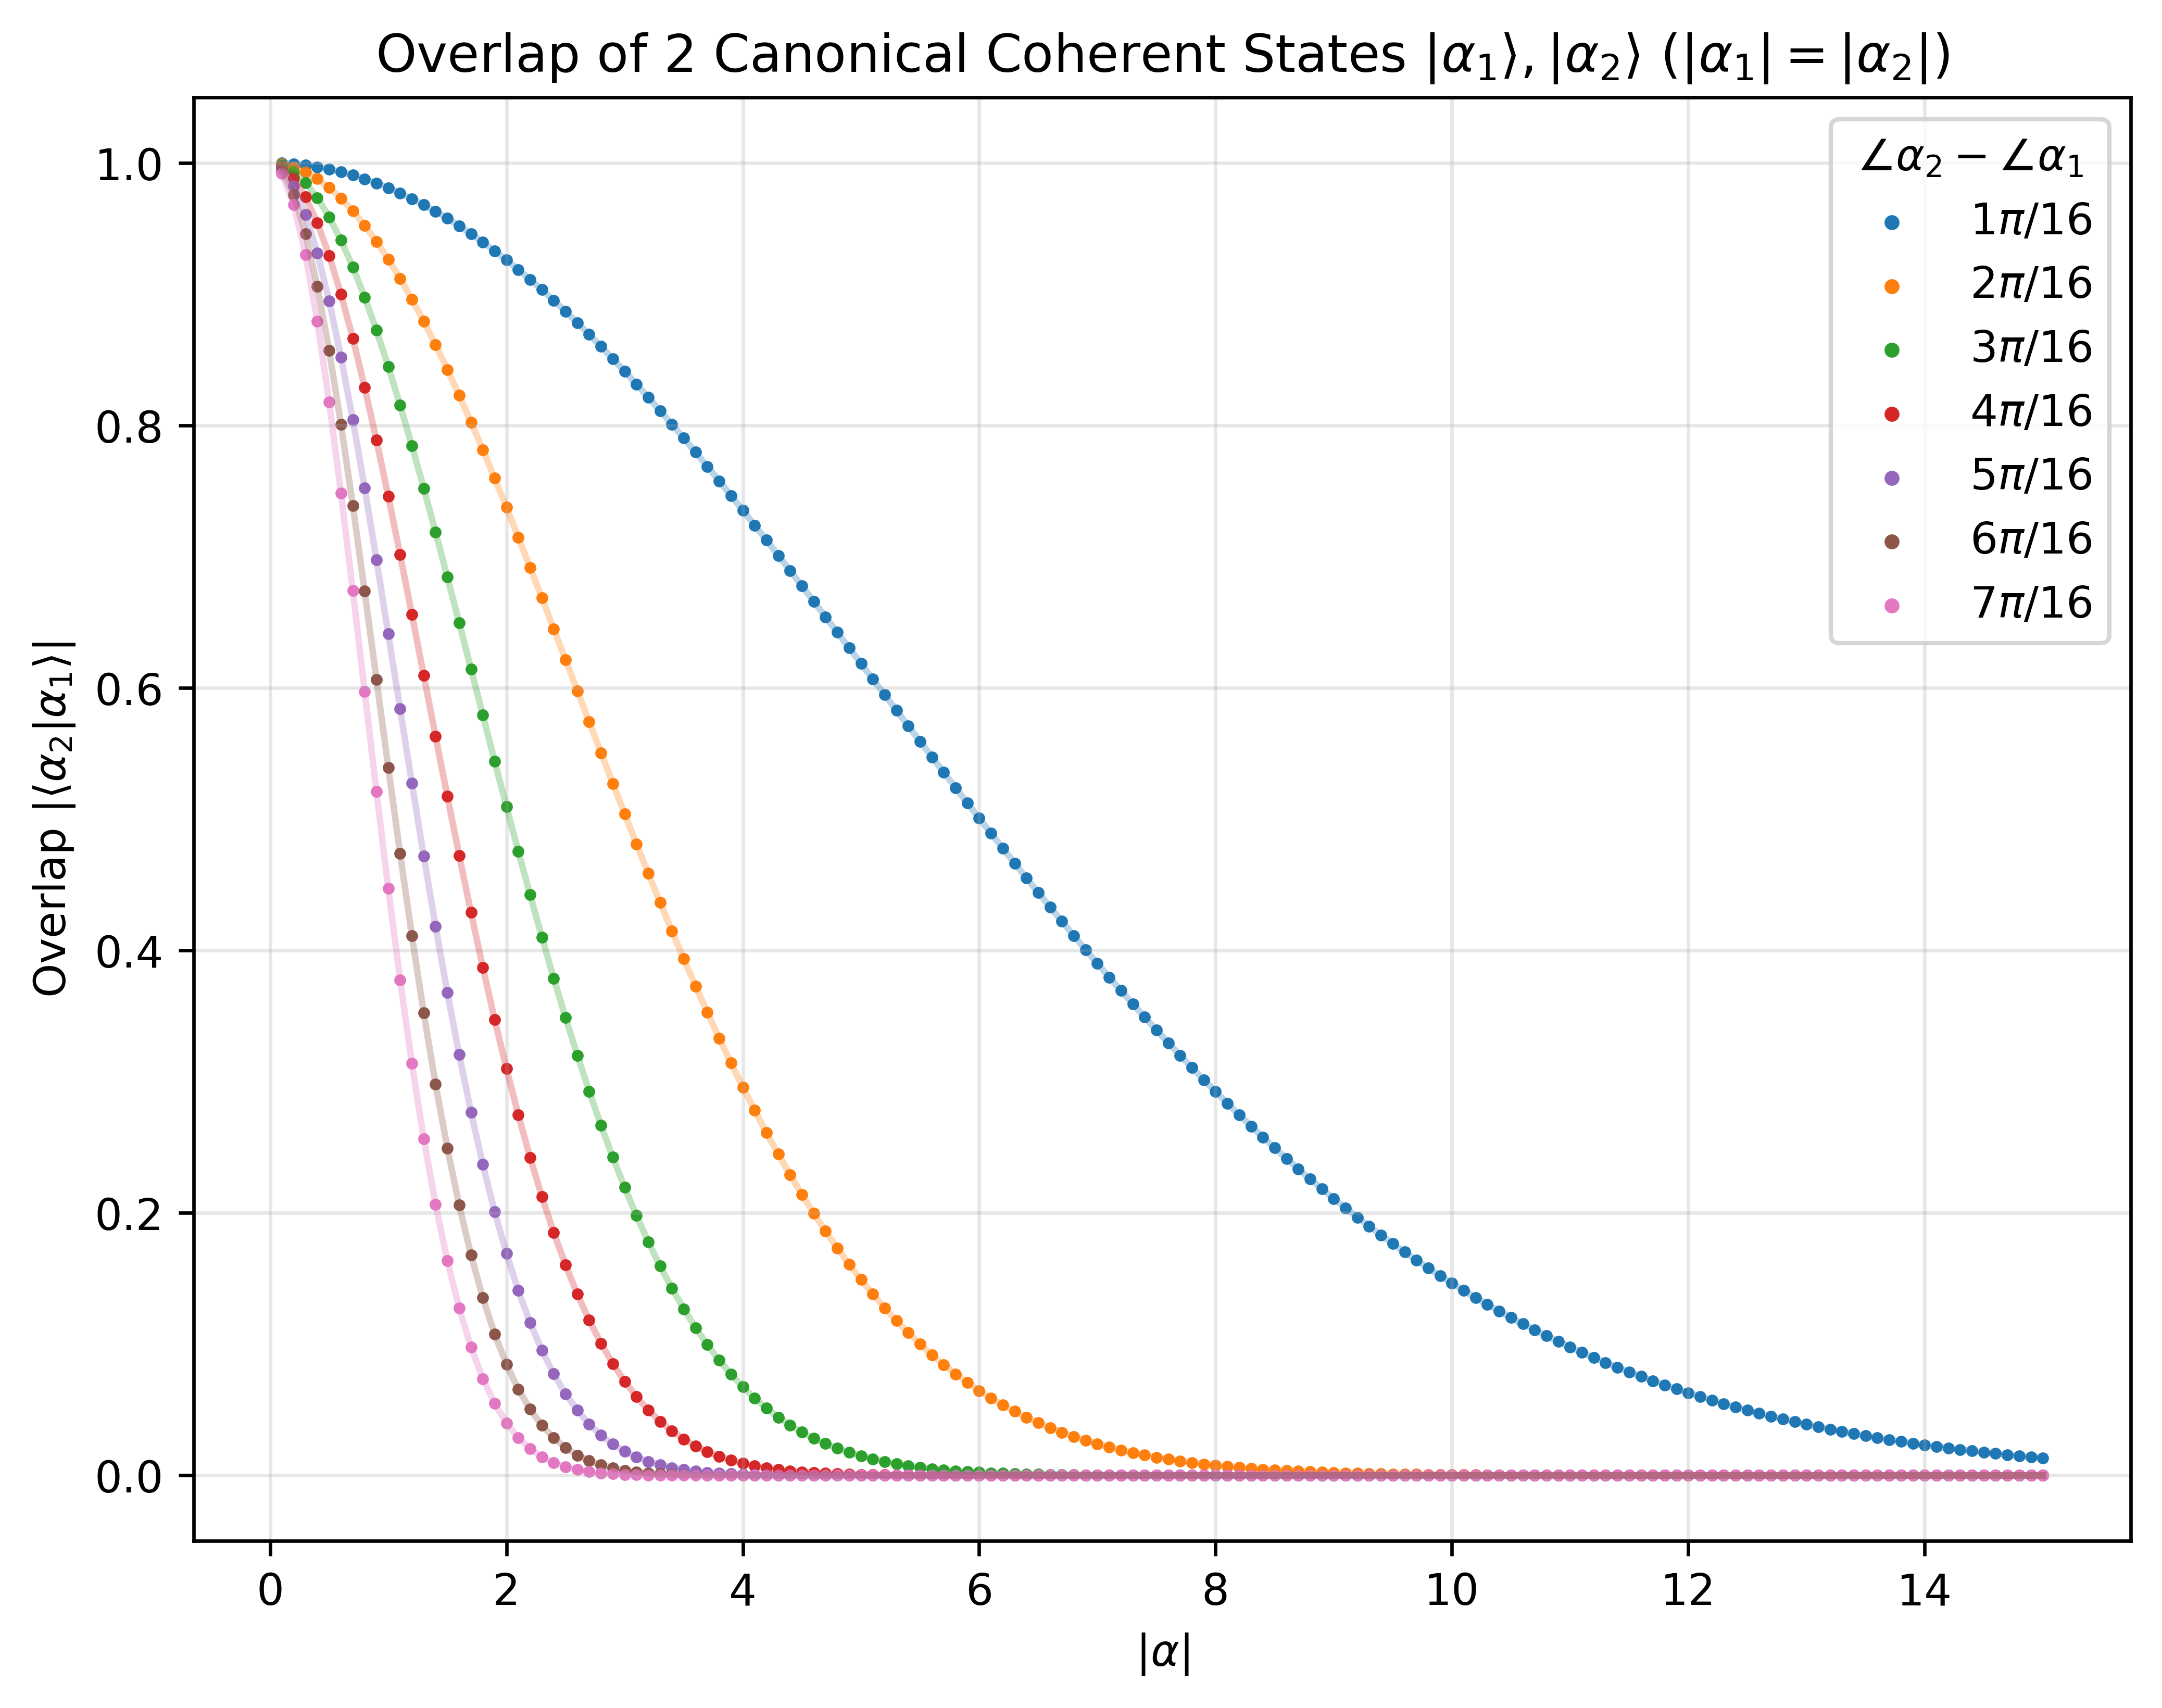
\includegraphics{figures/overlap.png}
    }
    \caption{Relationship between phase difference and state overlap for two coherent states with the same \(|\alpha|\).}
    \label{fig:coherent_overlap}
\end{figure}

\section{Quantum Measurement}
% Revised by Gemini 2.5 Flash
Quantum mechanics provides the fundamental framework for accurately describing
and predicting phenomena within physical systems.
Central to this framework is the concept of quantum measurement.
The third postulate of quantum mechanics \cite{qcqi} describes quantum measurements as follows:
\begin{quote}
    Quantum measurements are described by a collection ${M_{m}}$ of
    measurement operators. These are operators acting on the state space of the
    system being measured. The index $m$ refers to the measurement outcomes that
    may occur in the experiment. If the state of the quantum system is $\ket{\psi}$
    immediately before the measurement then the probability that result $m$ occurs is
    given by
    \begin{align}
        p(m) = \bra{\psi} M_{m}^{\dagger} M_{m}\ket{\psi}.
    \end{align}
    where $\Sigma_{m} M_{m}^{\dagger} M_{m} = I$.
\end{quote}

\subsection{Positive Operator-Valued Measure (POVM)}
\label{subsec:povm}

% Revised by Gemini 2.5 Flash
A POVM element $\Pi_{m}$ is defined as $\Pi_{m} \equiv M_{m}^{\dagger} M_{m}$.
A POVM is a complete set of positive-operator valued elements $\{\Pi_{m}\}$ that satisfies the following conditions:
\begin{itemize}
    \item Each $\Pi_{m}$ is a positive operator, i.e., $\bra{\psi}\Pi_m\ket{\psi} \ge 0$ for all $\ket{\psi}$.
    \item The elements satisfy the completeness relation: $\sum_{m} \Pi_{m} = I$.
    \item The probability of obtaining outcome $m$ when the system is in state $\ket{\psi}$ is given by $p(m) = \bra{\psi} \Pi_{m} \ket{\psi}$.
\end{itemize}
POVMs are essential for a complete description of quantum measurements,
particularly when considering the effect of a projective measurement performed
on a larger system that includes a subsystem of interest.
They are especially useful for characterizing measurements on subsystems of
entangled states or when the measurement device is itself part of a larger quantum system.

Figure \ref{fig:povm_pvm} illustrates the relationship between a Positive
Operator-Valued Measure (POVM) and a Projection-Valued Measure (PVM).
In this representation, $\rho_{1 + \text{anc}}$ denotes an extended system
comprising subsystem $\rho_1$ and one or more ancilla qubits, and $U$ represents a unitary operation.

\begin{figure}[htbp]
    \centering
    \scalebox{0.8}{
        \begin{quantikz}[column sep=0.5cm, row sep=0.4cm]
    & \lstick[3]{$\ket{\psi_1}$} & \qw & \gate[3]{\textsf{POVM}} & \qw \\
    & & \qw & \qw  & \qw                     \\
    & & \qw & \qw  & \qw                     \\
\end{quantikz}
\hspace{0.5cm}
$\equiv$
\begin{quantikz}[column sep=0.5cm, row sep=0.4cm]
    & \lstick[3]{$\ket{\psi_1}$} & \qw & \gate[5]{\textsf{PVM}} & \qw \\
    & & \qw & & \qw                     \\
    & & \qw & & \qw                     \\
    & \lstick[2]{$\ket{\psi_{anc}}$}      & \qw & \qw      & \qw            \\
    &      & \qw & \qw    & \qw          \\
\end{quantikz}
    }
    \caption{The relation between POVM and PVM.}
    \label{fig:povm_pvm}
\end{figure}

% \cite{10.5555/3240076}

\section{Quantum Isometry}
A fundamental concept in quantum mechanics that generalizes unitary evolution
is that of a quantum isometry.
While unitary operators describe the evolution of a closed quantum system where
the dimension of the input and output Hilbert spaces are the same, an isometry
provides a broader description for mappings where the output space can be larger than the input space.

Formally, a linear operator $V: \mathcal{H}_A \to \mathcal{H}_B$ from a Hilbert
space $\mathcal{H}_A$ to a Hilbert space $\mathcal{H}_B$ is an isometry if it
preserves the inner product, meaning $\braket{V\psi}{V\phi} = \braket{\psi}{\phi}$
for all states $\ket{\psi}, \ket{\phi} \in \mathcal{H}_A$.
This condition implies that $V^\dagger V = I_{\mathcal{H}_A}$, where
$I_{\mathcal{H}_A}$ is the identity operator on $\mathcal{H}_A$.
If $\mathcal{H}_A$ and $\mathcal{H}_B$ have the same dimension and the isometry
is surjective (i.e., $VV^\dagger = I_{\mathcal{H}_B}$), then the isometry is also a unitary operator.

Physically, isometries are crucial for describing the evolution of open quantum systems,
where a system of interest interacts with an external environment or auxiliary
system (often called an ancilla).
While the total system (system + ancilla) evolves unitarily, the evolution of
the system of interest alone, when viewed as a map from its initial state to
its final state, can be described by an isometry mapping its state space into
the larger combined space.
This concept lays the groundwork for understanding how generalized measurements
can arise from unitary dynamics and projective measurements on an expanded system.


\section{Naimark's Dilation Theorem}
\label{sec:naimark}
Naimark's dilation theorem is a cornerstone result in quantum information
theory that links generalized measurements (POVMs) to unitary evolution and projective measurements.
In essence, the theorem states that any POVM measurement can be realized as a projective measurement on a larger quantum system.
This larger system is constructed by augmenting the original system with an
additional, auxiliary quantum system, commonly referred to as an ancilla.

The core idea can be understood through a three-step process:
\begin{enumerate}
    \item \textbf{Introduce an Ancilla:} An auxiliary quantum system (ancilla), typically prepared in a known initial state (e.g., $\ket{0}_{\text{ancilla}}$), is coupled to the quantum system of interest.
    \item \textbf{Unitary Interaction:} The combined system (original system + ancilla) then undergoes a global unitary evolution. This interaction entangles the original system with the ancilla.
    \item \textbf{Projective Measurement:} A standard projective measurement is subsequently performed on the combined system, or often, just on the ancilla component.
\end{enumerate}
Remarkably, the probabilities of obtaining different outcomes for the original system, and its post-measurement state, are precisely identical to those that would be obtained by directly performing the initial POVM.

This theorem has profound implications for both the theory and practice of quantum mechanics.
It demonstrates the universality of projective measurements, showing that even
the most general and complex measurements (POVMs), which may describe noisy or
incomplete measurements on a subsystem, can always be simulated by a sequence
of elementary unitary operations and projective measurements on a larger, closed system.
This theoretical equivalence is vital for understanding the physical
implementation of quantum measurements and for developing general theories of
quantum operations.

% Chapter 2 of \cite{10.5555/3240076}
% \cite{RN12}.

\section{Noise model}

The experimental environment is not perfect. To model the imperfections that
appear in quantum communication or quantum circuits, different noise models
have been proposed. Chapter 8.3 of \cite{qcqi}
Among the We use the depolarizing channel as the noise model.
The depolarizing channel assumes that the information of the qubits disappear over time.
The depolarizing channel is a generalization of the bit flip, phase flip, and bit-phase flip channels.

Our assumptions on the system environment will affect where we apply the noise
models. Sometimes we add the depolarizing channel direct to our input states
and sometimes we make an assumption that a depolarizing channel is present
after executing certain quantum gates.

\section{Quantum circuits}

In this section, we will briefly introduce the keys elements of the quantum
circuit model, in the hope to make the thesis more self-contained. Readers may
refer to Chapter 4 in \cite{qcqi} for more details.


The basis gate set for ibm\_blah is

\section{Other properties}
\subsection{State Fidelity}
\label{subsec:state_fid}
State fidelity is a measure of similarity between two quantum states, crucial
for evaluating the accuracy of state approximations in quantum state
discrimination tasks.
For two density matrices \(\rho_1\) and \(\rho_2\), the state fidelity
\(F(\rho_1, \rho_2)\) is defined as
\begin{align}
    F(\rho_1, \rho_2) = \left( \operatorname{Tr} \left[ \sqrt{\sqrt{\rho_1} \rho_2 \sqrt{\rho_1}} \right] \right)^2.
\end{align}
When \(\rho_1 = |\psi_1\rangle\langle\psi_1|\) is a pure state, this simplifies to
\begin{align}
    F(\rho_1, \rho_2) = \langle \psi_1 | \rho_2 | \psi_1 \rangle.
\end{align}
In this thesis, state fidelity is used to quantify the similarity between a
truncated coherent state (padded to 10 qubits) and an ideal coherent state
truncated to 10 qubits, as discussed in Chapter \ref{chap:qc_qsd}.
This metric ensures that our approximations of coherent states are
sufficiently accurate for reliable discrimination in noisy environments.

\subsection{Process Fidelity}
\label{subsec:proc_fid}
Process fidelity quantifies the similarity between two quantum channels,
essential for assessing the performance of synthesized quantum circuits
against their ideal counterparts.
For quantum channels \(\mathcal{E}\) and \(\mathcal{F}\), the process fidelity
\(F_{\text{pro}}(\mathcal{E}, \mathcal{F})\) is defined as
\begin{align}
    F_{\text{pro}}(\mathcal{E}, \mathcal{F}) = F(\rho_{\mathcal{E}}, \rho_{\mathcal{F}}),
\end{align}
where \(F\) is the state fidelity, \(\rho_{\mathcal{E}} = \Lambda_{\mathcal{E}} / d\)
is the normalized Choi matrix of channel \(\mathcal{E}\), and \(d\) is the
input dimension of \(\mathcal{E}\).
When the target channel is a unitary \(U\), this becomes
\begin{align}
    F_{\text{pro}}(\mathcal{E}, U) = \frac{\operatorname{Tr}[S_U^\dagger S_{\mathcal{E}}]}{d^2},
\end{align}
where \(S_{\mathcal{E}}\) and \(S_U\) are the superoperator matrices for
\(\mathcal{E}\) and \(U\), respectively, and \(d\) is the input dimension.
In Chapter \ref{chap:qc_qsd}, process fidelity is employed to compare the
unitary matrix of an optimized quantum circuit with that of the original
circuit, ensuring that circuit simplifications preserve the intended
discrimination functionality.
